% IPIS Module 3 -- manuscript for The Canadian Journal of Chemical Engineering (regular article)
% Build: pdflatex main && bibtex main && pdflatex main && pdflatex main
\documentclass[12pt]{article}
\usepackage[letterpaper,margin=2.5cm]{geometry}
\usepackage[T1]{fontenc}
\usepackage{mathptmx}
\usepackage{amsmath,amsthm}
\usepackage{graphicx}
\usepackage{booktabs}
\usepackage{array}
\usepackage[numbers,super,sort&compress]{natbib}
\setcitestyle{open={[},close={]}}
\usepackage{setspace}
\usepackage{lineno}
\usepackage{ragged2e}
\usepackage{caption}
\captionsetup[figure]{labelfont=bf,name=FIGURE,labelsep=space}
\captionsetup[table]{labelfont=bf,name=TABLE,labelsep=space,position=top}
\usepackage[hidelinks]{hyperref}
\newtheorem{proposition}{Proposition}
\onehalfspacing
\linenumbers

\newcommand{\affil}{Mapua Malayan Colleges Mindanao, Davao City, Philippines}

\begin{document}

\setlength{\RaggedRightRightskip}{0pt plus 6em}
\RaggedRight
\begin{center}
{\large\bfseries Safe real-time optimization of a distillation column under feed-composition
uncertainty: a comparative study of distribution-free constraint back-offs}\\[10pt]
Bien Don Busico\\[2pt]
{\small Mapua Malayan Colleges Mindanao, Davao City, Davao del Sur, Philippines}
\end{center}
\noindent\textbf{Correspondence}\\
\noindent Bien Don Busico, Mapua Malayan Colleges Mindanao, Davao City, Davao del Sur,
Philippines.\\ Email: bienbusico@gmail.com

\begin{abstract}\singlespacing
\noindent Real-time optimization (RTO) pushes a distillation column toward its product
specifications, so the optimizer must subtract a back-off from any specification it cannot
measure online. Data-driven back-offs sized with conformal prediction are attractive because they
need no disturbance model, but their guarantee holds on average over operating points, and the
optimizer does not choose operating points at random. This study compares six ways of sizing the
back-off of a chance-constrained RTO for a rigorous DWSIM Peng-Robinson debutanizer twin under an
unmeasured feed-composition disturbance, scoring every deployed setpoint by its exact violation
probability over 1000 repeated trials. At the realistic disturbance level, conformal back-offs
that are valid on average deploy a setpoint whose violation probability exceeds the 10\% target in
67.5\% to 100\% of trials, and an a posteriori plug-in correction still does so in 32.0\%.
Certify-then-deploy, a fixed-sequence binomial test of candidate setpoints, and scenario-based
sampling-and-discarding keep this rate at or below 2.5\% while staying within 0.06\% to 0.21\% of the
oracle profit. A risk-adjusted analysis shows that the unguaranteed back-offs lose money in
expectation once off-spec bottoms cost more than 0.017 to 0.032 USD/kg, about 2\% to 4\% of the
product value. The results give a selection rule: use sampling-and-discarding when the plant model
fits inside the optimizer, and certify-then-deploy when it does not.
\end{abstract}

\noindent\textbf{Keywords:} chance constraint, conformal prediction, digital twin, distillation,
real-time optimization, scenario approach

\section{INTRODUCTION}

Real-time optimization (RTO) recomputes the setpoints of a process unit as prices, feeds, and
equipment drift, and it earns its value by operating closer to constraints than a fixed recipe
would. In a debutanizer the most profitable operation keeps as much material as possible in the
more valuable stream, which drives the bottoms composition toward its specification. That
specification is usually not measured online. It is known through laboratory analyses or an
inferential estimate, so the optimizer must subtract a back-off from the specification to protect
against disturbances it cannot see. The back-off is the central design quantity of RTO under
uncertainty: too small and the column produces off-spec product whenever the disturbance is
adverse; too large and the economic benefit of the optimization is given away. Adaptation schemes
correct the optimizer for plant-model mismatch,\citep{marchetti2009,chachuat2009} and
data-driven models of distillation columns have recently been placed inside RTO loops,\citep{rodriguez2025cjce} but both still need a principled rule for sizing the margin on an
unmeasured quality.

The classical rule is a chance constraint, which bounds the probability of violating the
specification under an assumed disturbance distribution.\citep{li2008} Distribution-free
alternatives remove that assumption. Conformal prediction turns any predictor into an interval
whose coverage holds in finite samples when the data are exchangeable, without a model of the
disturbance\citep{vovk2005,lei2018,angelopoulos2023}; conformalized quantile regression adapts the
interval width to the operating point.\citep{romano2019} Placing the upper edge of such an
interval as the back-off is therefore a natural way to size the margin from plant or simulator
data, and conformal constructions have recently been proposed inside optimization and control.\citep{zhao2024cpp,zhang2024}

Back-offs themselves are well established in process systems engineering. Stochastic back-off
algorithms size margins for integrated design, control, and scheduling under uncertainty\citep{rafiei2018,koller2018}; explicit back-offs tighten the constraints of stochastic nonlinear
model predictive control\citep{paulson2018,mesbah2016}; Gaussian-process models supply back-offs
in data-driven predictive control\citep{bradford2020}; and back-offs can be tuned by Bayesian
optimization from the empirical distribution of constraint values.\citep{petsagkourakis2022} Each
of these studies proposes and evaluates one construction. Conformal prediction has also been
linked to scenario optimization at the level of guarantees,\citep{osullivan2025,campi2009} and
conformal constraint learning has been proposed for mixed-integer design.\citep{ovalle2025}

The difficulty is that conformal coverage is a statement about an average. It holds over the
distribution of operating points used for calibration, while an optimizer deliberately seeks the
boundary of the feasible region, where the margin is tightest relative to the local risk. Selecting
the best point by optimization favours exactly the points where the margin is optimistic, an
instance of the optimizer's curse known in decision analysis,\citep{smith2006} and coverage
conditional on the chosen operating point cannot be guaranteed without further structure.\citep{foygelbarber2021} Remedies exist in the statistics and control literature: calibrating the
chosen solution again on an independent sample,\citep{zhao2024cpp} tuning a margin by
fixed-sequence testing,\citep{angelopoulos2021ltt,einbinder2025} and the scenario approach with
its sampling-and-discarding variant.\citep{calafiore2006,campi2008,campi2011} What a process
engineer lacks is a like-for-like comparison of these options on a rigorous process model, with the
consequences stated in the units that matter in a plant: how often an unsafe setpoint is actually
deployed, what the guarantee costs in profit, and which option to use in which situation.

This paper supplies that comparison. No new method is proposed, and the contribution is stated
accordingly. To the author's knowledge, this is the first controlled head-to-head comparison of
distribution-free back-off constructions (split conformal, conformalized quantile regression, an a
posteriori plug-in correction, fixed-sequence certify-then-deploy, the scenario approach, and
sampling-and-discarding) for chance-constrained steady-state RTO of a distillation column. The
novel elements are (i) exact violation scoring of every deployed setpoint over 1000 repeated trials
on a rigorous DWSIM Peng-Robinson twin, (ii) the rate at which each construction deploys an unsafe
setpoint across a range of disturbance magnitudes, (iii) a risk-adjusted economic analysis that
converts the safety differences into a breakeven off-spec cost, and (iv) a selection rule and a
certification-budget table that can be applied before commissioning. Section
2 states the problem, Section 3 the constructions compared, Section 4 the twin and the experiment,
Section 5 the results, and Section 6 the selection guide and limitations.

\section{PROBLEM FORMULATION}

The decision is the operating point $u=(R,D)$, with $R$ the reflux ratio and $D$ the distillate
flow in kmol/h, restricted to the box $0.8 \le R \le 3.0$, $33 \le D \le 37$. The disturbance $z$
is the \textit{n}-butane mole fraction of the feed. It is neither manipulated nor measured online, and its
distribution $P$ is unknown to the optimizer; successive values are treated as independent draws
over the RTO time scale. The constrained quality is the bottoms \textit{n}-butane mole fraction
$g(u,z)=x_B$, with specification $x_B \le \bar g = 0.02$. The operating profit $\pi(u)$ values the
overhead at the liquefied petroleum gas price and the bottoms at the stabilized-gasoline price, both
by mass, less the reboiler energy cost.

The chance-constrained RTO is formulated as follows:
\begin{equation}
\max_{u}\ \pi(u) \quad \text{s.t.} \quad P\!\left(g(u,z) \le \bar g\right) \ge 1-\alpha ,
\label{eq:cc}
\end{equation}
with $\alpha = 0.10$. Writing $V(u) = P(g(u,z) > \bar g)$ for the violation probability of a
setpoint, the constraint reads $V(u) \le \alpha$. Because $V$ is not available, the optimizer uses
a nominal model $\hat g(u) = g(u, z_0)$ at the nominal composition $z_0=0.35$ and a back-off
$C(u) \ge 0$ as follows:
\begin{equation}
\max_{u}\ \pi(u) \quad \text{s.t.} \quad \hat g(u) + C(u) \le \bar g .
\label{eq:backoff}
\end{equation}
Two kinds of guarantee must be distinguished. A back-off is \emph{marginally valid} if the
probability that $g$ exceeds $\hat g + C$ is at most $\alpha$ on average over the operating points
used to calibrate it. The engineering requirement is different: the plant runs at the one setpoint
the optimizer deploys, so what matters is whether that setpoint satisfies $V \le \alpha$. This
paper therefore judges every method by the deployed-decision criterion as follows:
\begin{equation}
P\!\left(V(u_{\mathrm{dep}}) > \alpha\right] \le \delta ,
\label{eq:pac}
\end{equation}
with $\delta=0.05$, where the probability is over the data used to build and check the back-off.

\section{BACK-OFF CONSTRUCTIONS COMPARED}

\subsection{Marginal conformal back-offs}
A calibration set $\{(u_i,z_i,g_i)\}_{i=1}^n$ of evaluations at random operating points gives
residuals $r_i = g_i - \hat g(u_i)$. The \emph{fixed} back-off is the one-sided split-conformal
quantile of the residuals, $C = r_{(q)}$ with $q = \lceil (n+1)(1-\alpha) \rceil$\citep{vovk2005,lei2018}; it spends the same margin everywhere. The \emph{conformalized quantile
regression} (CQR) back-off fits a gradient-boosted estimate $\hat q(u)$ of the conditional
$(1-\alpha)$ quantile of $g$ and adds the conformal quantile of $g_i - \hat q(u_i)$,\citep{romano2019} so its width follows the local risk. Both are marginally valid; neither is
guaranteed at the setpoint the optimizer selects.

\subsection{A posteriori plug-in correction}
A common repair solves Equation~\eqref{eq:backoff} with the CQR back-off, then inflates it by the smallest
factor $\kappa \ge 1$ whose resulting setpoint meets the target on a validation sample of
disturbances, in the spirit of the a posteriori calibration of conformal predictive programming.\citep{zhao2024cpp} In the implementation compared here the validation sample has 6000 draws and a
tolerance of 0.01 is allowed. The correction is accurate on average, but $\kappa$ is chosen with the
same sample that judges it, so it carries no guarantee of the form Equation~\eqref{eq:pac}.

\subsection{Certify-then-deploy}
Certify-then-deploy separates choosing candidates from checking them. For a decreasing list
$\kappa_1 > \kappa_2 > \dots > \kappa_J$ fixed in advance, the optimizer produces candidate
setpoints $u_j$ by solving Equation~\eqref{eq:backoff} with $\kappa_j C_{\mathrm{CQR}}$. An independent
certification sample $z'_1,\dots,z'_m$ is then drawn and each candidate is evaluated on it, giving
the violation count $N_j$. The one-sided Clopper-Pearson upper bound $U_j$ on $V(u_j)$ at
confidence $1-\delta$ is computed from $N_j$.\citep{clopper1934} Candidates are tested in order,
from the most conservative, and testing stops at the first candidate with $U_j > \alpha$; the last
candidate that passed is deployed, and if none passes the plant stays at a conservative fallback
setpoint.

\begin{proposition}
If the certification sample is independent of everything used to produce the candidates, then
$P(\text{a setpoint with } V > \alpha \text{ is deployed}) \le \delta$, whatever the model,
optimizer, or back-off used to produce the candidates.
\end{proposition}

\begin{proof}
Conditional on the candidates, $N_j$ is binomial with parameters $m$ and $V(u_j)$, so
$P(U_j < V(u_j)) \le \delta$ for each $j$. Let $j^\dagger$ be the first candidate with
$V(u_{j^\dagger}) > \alpha$. Because testing stops at the first failure, an unsafe candidate can be
deployed only if candidate $j^\dagger$ passes, that is, only if $U_{j^\dagger} \le \alpha <
V(u_{j^\dagger})$, which has probability at most $\delta$.
\end{proof}

This is the fixed-sequence argument used for risk control in Learn-then-Test.\citep{angelopoulos2021ltt} It needs no multiplicity correction and no convexity, and the sample
size $m$ does not depend on the number of decision variables. It does require that the plant model
$g$ can be evaluated at the candidate setpoints, which is the case for a validated simulator or for
pilot runs at the candidate conditions.

\subsection{Scenario approach and sampling-and-discarding}
The scenario approach imposes $g(u,z_i) \le \bar g$ for $N$ sampled disturbances. With two decision
variables, $N = 46$ gives $P(V > 0.10) \le 0.05$.\citep{calafiore2006,campi2008}
Sampling-and-discarding draws more scenarios and removes the $k$ most restrictive ones while keeping
the same guarantee\citep{campi2011}; with $N=1000$, $k=69$. Both evaluate the plant model inside
the optimizer.

\subsection{Oracle}
The oracle knows the disturbance distribution, sets $C(u) = g(u, z_{1-\alpha}) - \hat g(u)$ with
$z_{1-\alpha}$ the $(1-\alpha)$ quantile of $z$ (valid because $x_B$ increases with $z$), and serves
only as the reference.

\section{CASE STUDY AND EXPERIMENTAL DESIGN}

\subsection{Digital twin}
The plant is a DWSIM 9.0.5\citep{dwsim} model of a debutanizer reduced to the binary system
\textit{n}-butane/\textit{n}-hexane under the Peng-Robinson equation of state\citep{peng1976}: nine equilibrium
stages with the condenser as stage 0 and the reboiler as stage 8, feed on stage 4, top pressure
470 kPa (4.7 bar) with a 40 kPa (0.4 bar)
column pressure drop, and a feed of 100 kmol/h. A nominal campaign at $z_0 = 0.35$
covers a $4 \times 4$ grid of $R \in \{0.8, 1.5, 2.2, 3.0\}$ and $D \in \{33, 34.5, 36, 37\}$ kmol/h
(15 converged runs), and a disturbance campaign repeats the grid at
$z \in \{0.300, 0.325, 0.350, 0.375, 0.400\}$ (78 runs). Gaussian-process surrogates fitted to the
nominal runs give $\hat g$, the distillate purity, and the reboiler duty; a Gaussian process over
$(R, D, z)$ fitted to the disturbance campaign serves as the truth $g$. Leaving out the whole
$z=0.375$ slice and predicting it gives $R^2 = 0.917$ and a mean absolute error of 0.0053 in $x_B$.
Figure~\ref{fig:loop} shows the loop.

\begin{figure}[t]
\centering
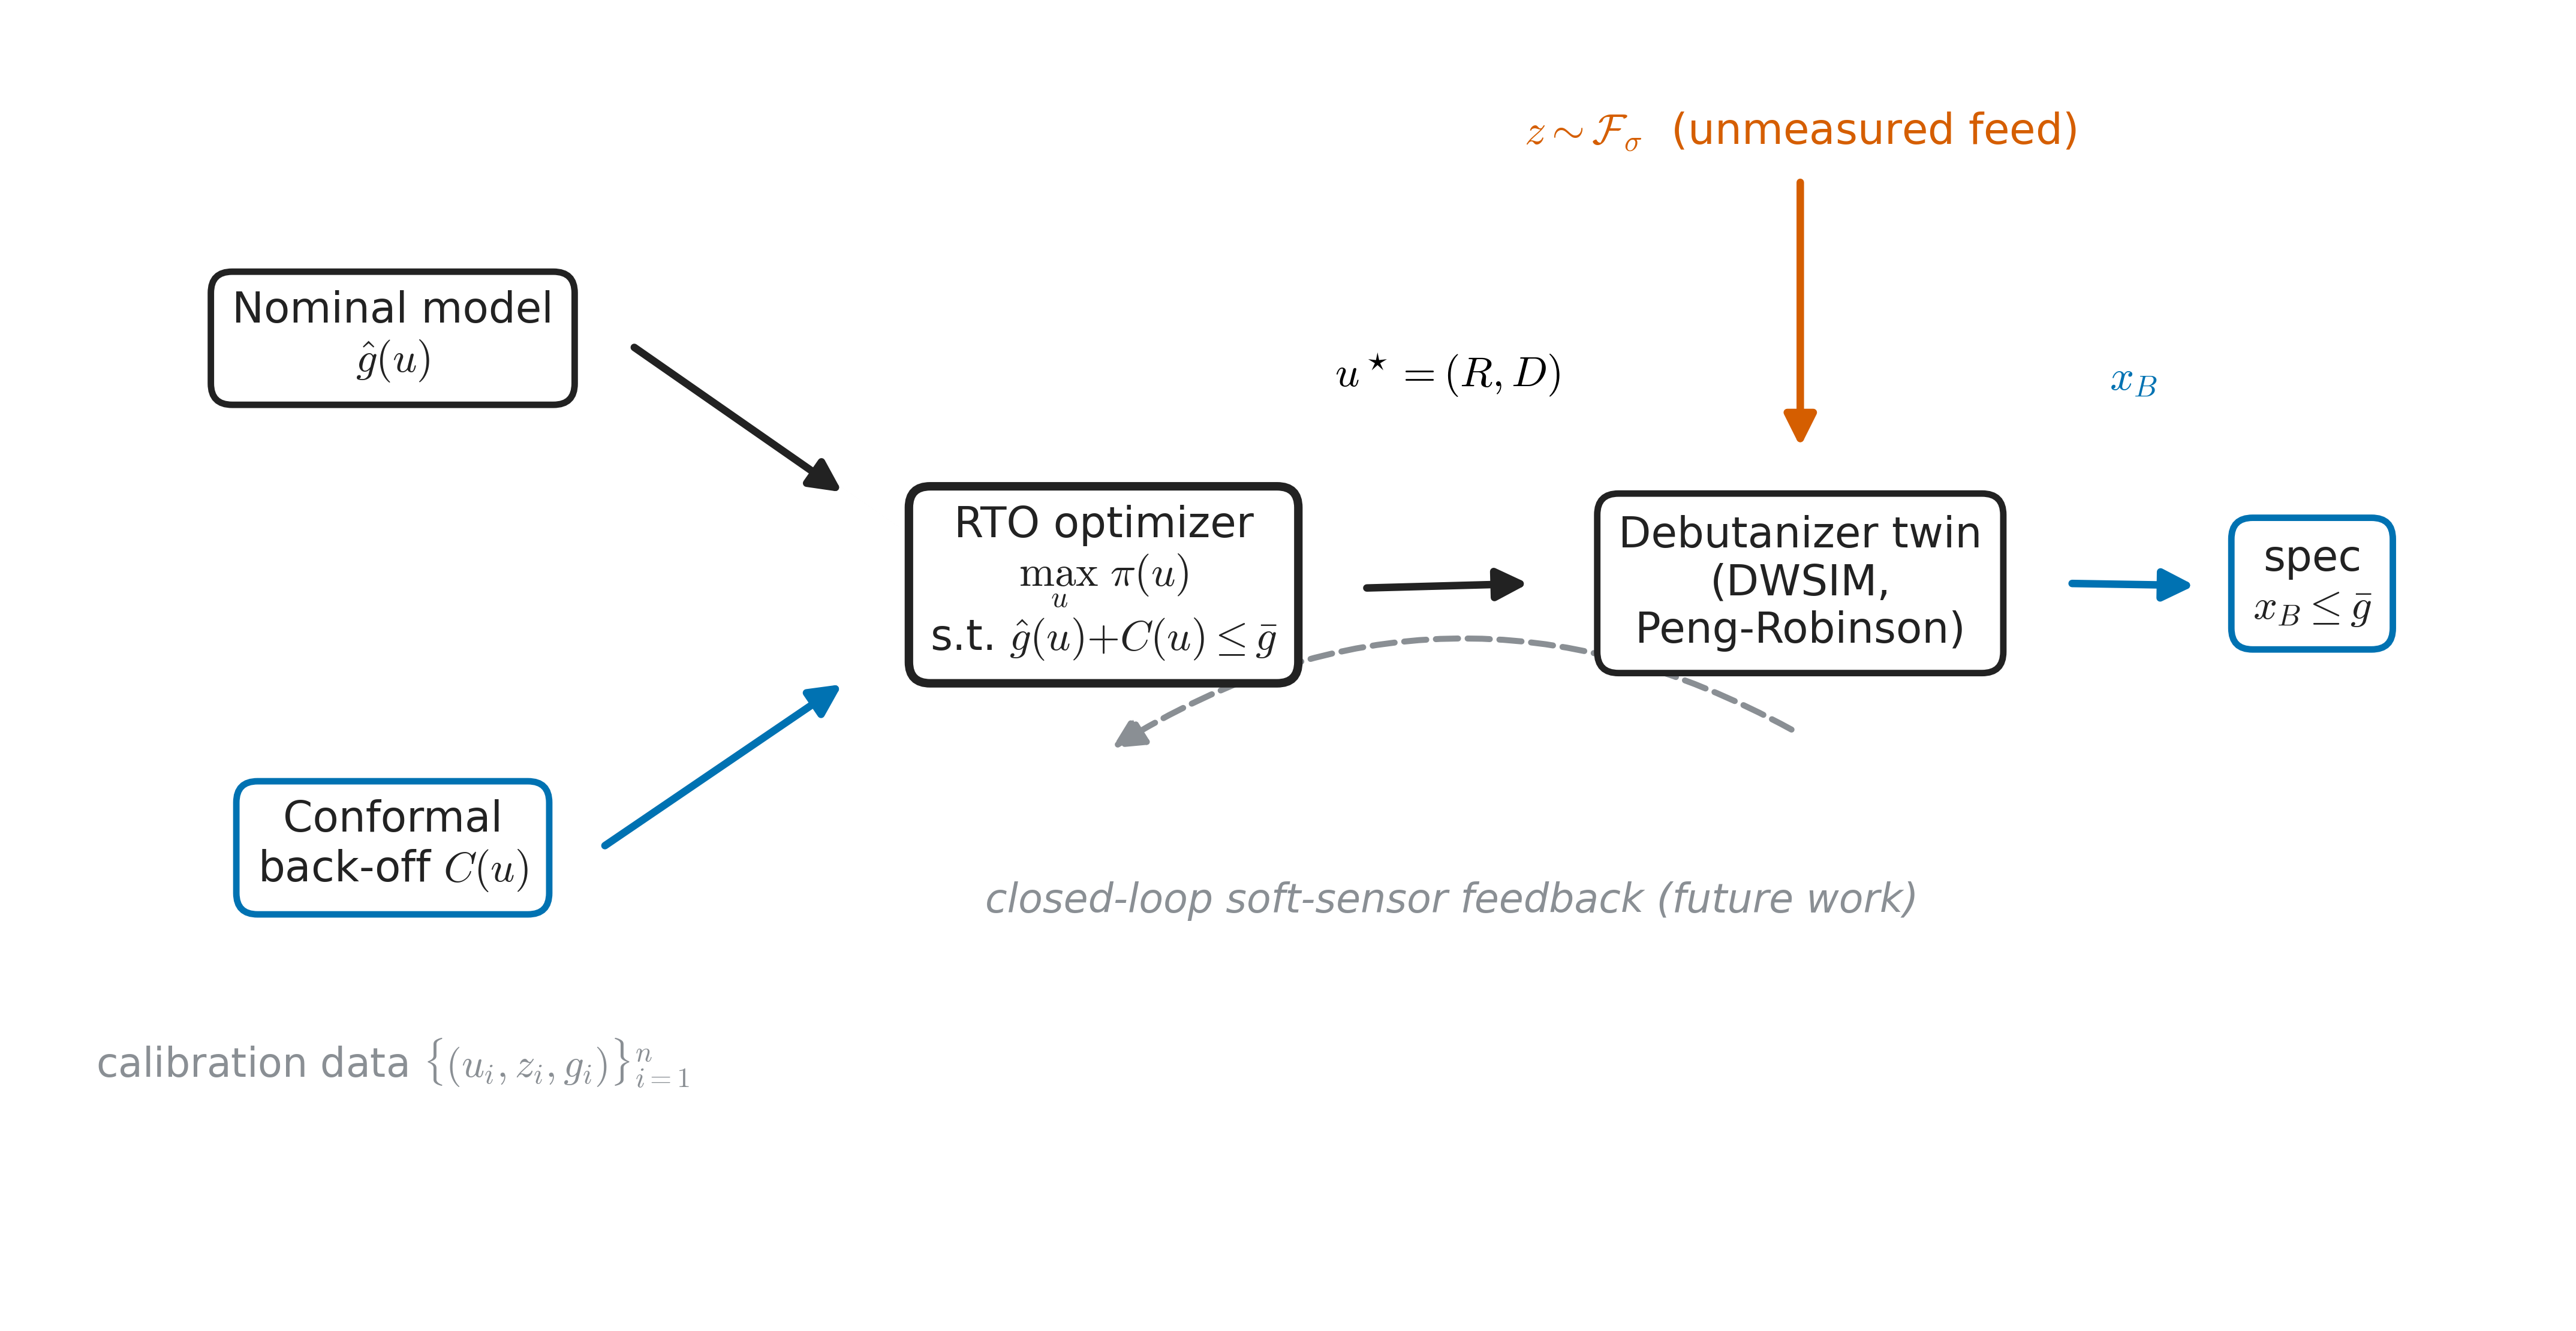
\includegraphics[width=\textwidth]{F1_rto_loop.png}
\caption{Chance-constrained real-time optimization (RTO) with a data-driven back-off. The optimizer uses the nominal model
and the back-off; the feed composition $z$ is not measured, and neither is the bottoms composition
$x_B$ it constrains.}
\label{fig:loop}
\end{figure}

\subsection{Economics}
Overhead is valued at the liquefied petroleum gas price (0.340 USD/kg) and bottoms at the
stabilized-gasoline price (0.836 USD/kg), and reboiler energy costs 6.28 USD/GJ. Because the
gasoline outvalues the light key, profit rises as the column lets more material leave with the
bottoms, which pushes $x_B$ toward its specification and makes the chance constraint economically
active.

\subsection{Experiment}
The optimizer is an exact search over a $67 \times 61$ grid of $(R, D)$ (4087 setpoints), so no
method is advantaged by a local solver. The feed composition is a normal variable centred on 0.35
and truncated to the campaign range of 0.30 to 0.40, with standard deviation
$\sigma_z$ of 0.006, 0.010, 0.015, 0.020, or 0.025; 0.006 is the realistic level for a
well-controlled feed. The calibration set has $n = 1500\max(1, \sigma_z/0.006)$ points. Each method
is run in 200 independent trials per $\sigma_z$ (1000 trials in total), with certification budgets
$m$ of 200 or 1000. Because $x_B$ increases with $z$ at 99.6\% of the grid setpoints, the
violation probability of any setpoint follows exactly from the composition at which it crosses the
specification, so every deployed setpoint is scored without Monte Carlo error.

For the economic comparison, the risk-adjusted profit rate of a setpoint is defined as follows:
\begin{equation}
J(u) = \pi(u) - \Delta\, \dot m_B\, V(u),
\label{eq:J}
\end{equation}
where $\Delta$ is the cost per kilogram of off-spec bottoms (downgrading or reprocessing) and
$\dot m_B = 5636$ kg/h is the bottoms flow at the oracle setpoint. A trial in which a method
abstains is charged the conservative fallback setpoint, the most profitable one with $V \le 0.01$.

A synthetic benchmark with an exactly known violation probability (two decision variables, a skewed
disturbance, sensitivity that grows in the profitable direction, 400 trials) is used to isolate the
mechanism behind the failure of marginal back-offs; the code for both studies is public. Portions of
the analysis and plotting code were written with the assistance of a large language model (see
Acknowledgements); the author reviewed and tested all code, and every reported number regenerates
from the public scripts and fixed random seeds.

\subsection{Use of generative artificial intelligence tools}
The author used Claude (Anthropic; Claude Opus 5.5 and earlier versions), a large language model,
to assist with drafting and editing the manuscript text and with writing and debugging parts of the
Python analysis and plotting code. The author directed the study, reviewed and tested all outputs,
verified every reported number against the regenerated evidence files, and takes full
responsibility for the content. No generative AI tool was used to create or alter simulation data
or results; the figures were produced by the author's code from the simulation data.

\section{RESULTS AND DISCUSSION}

\subsection{Why valid-on-average back-offs fail under optimization}
In the synthetic benchmark the fixed, normalized, and CQR back-offs all reach their marginal
target exactly (average miss 0.100), yet the setpoint the optimizer selects is unsafe in 93\% to
100\% of trials, with a violation probability of 0.17 to 0.18. The cause is selection. The
normalized back-off scales the margin by a local estimate of the residual spread; when that
estimate is made noisier (fewer neighbours in a nearest-neighbour estimate), unsafe deployments rise
from 61.0\% to 99.7\%, and even the smoothest estimate stays far above $\delta$. An estimate that is
unbiased everywhere is still optimistic somewhere, and the optimizer finds that place. In the same
benchmark certify-then-deploy deploys an unsafe setpoint in 1.5\% of trials (95\% interval 0.6\% to
3.2\%), consistent with the proposition.

\subsection{Safety on the distillation twin}
Figure~\ref{fig:unsafe} and Table~\ref{tab:main} give the twin results. At the realistic
disturbance ($\sigma_z = 0.006$), the fixed conformal back-off deploys an unsafe setpoint in every
trial and the CQR back-off in 67.5\% of trials, with expected violation probabilities of 0.157 and
0.147 against a target of 0.10. The a posteriori plug-in correction lowers the expected violation
to 0.073, close to the target on average, but still deploys an unsafe setpoint in 32.0\% of trials;
across all disturbance levels this rate ranges from 12.0\% to 35.5\%. An average that looks right is
not a guarantee. Certify-then-deploy keeps unsafe deployments at or below 2.5\% at every
disturbance level and both budgets, and sampling-and-discarding at or below 0.5\%.

\begin{figure}[t]
\centering
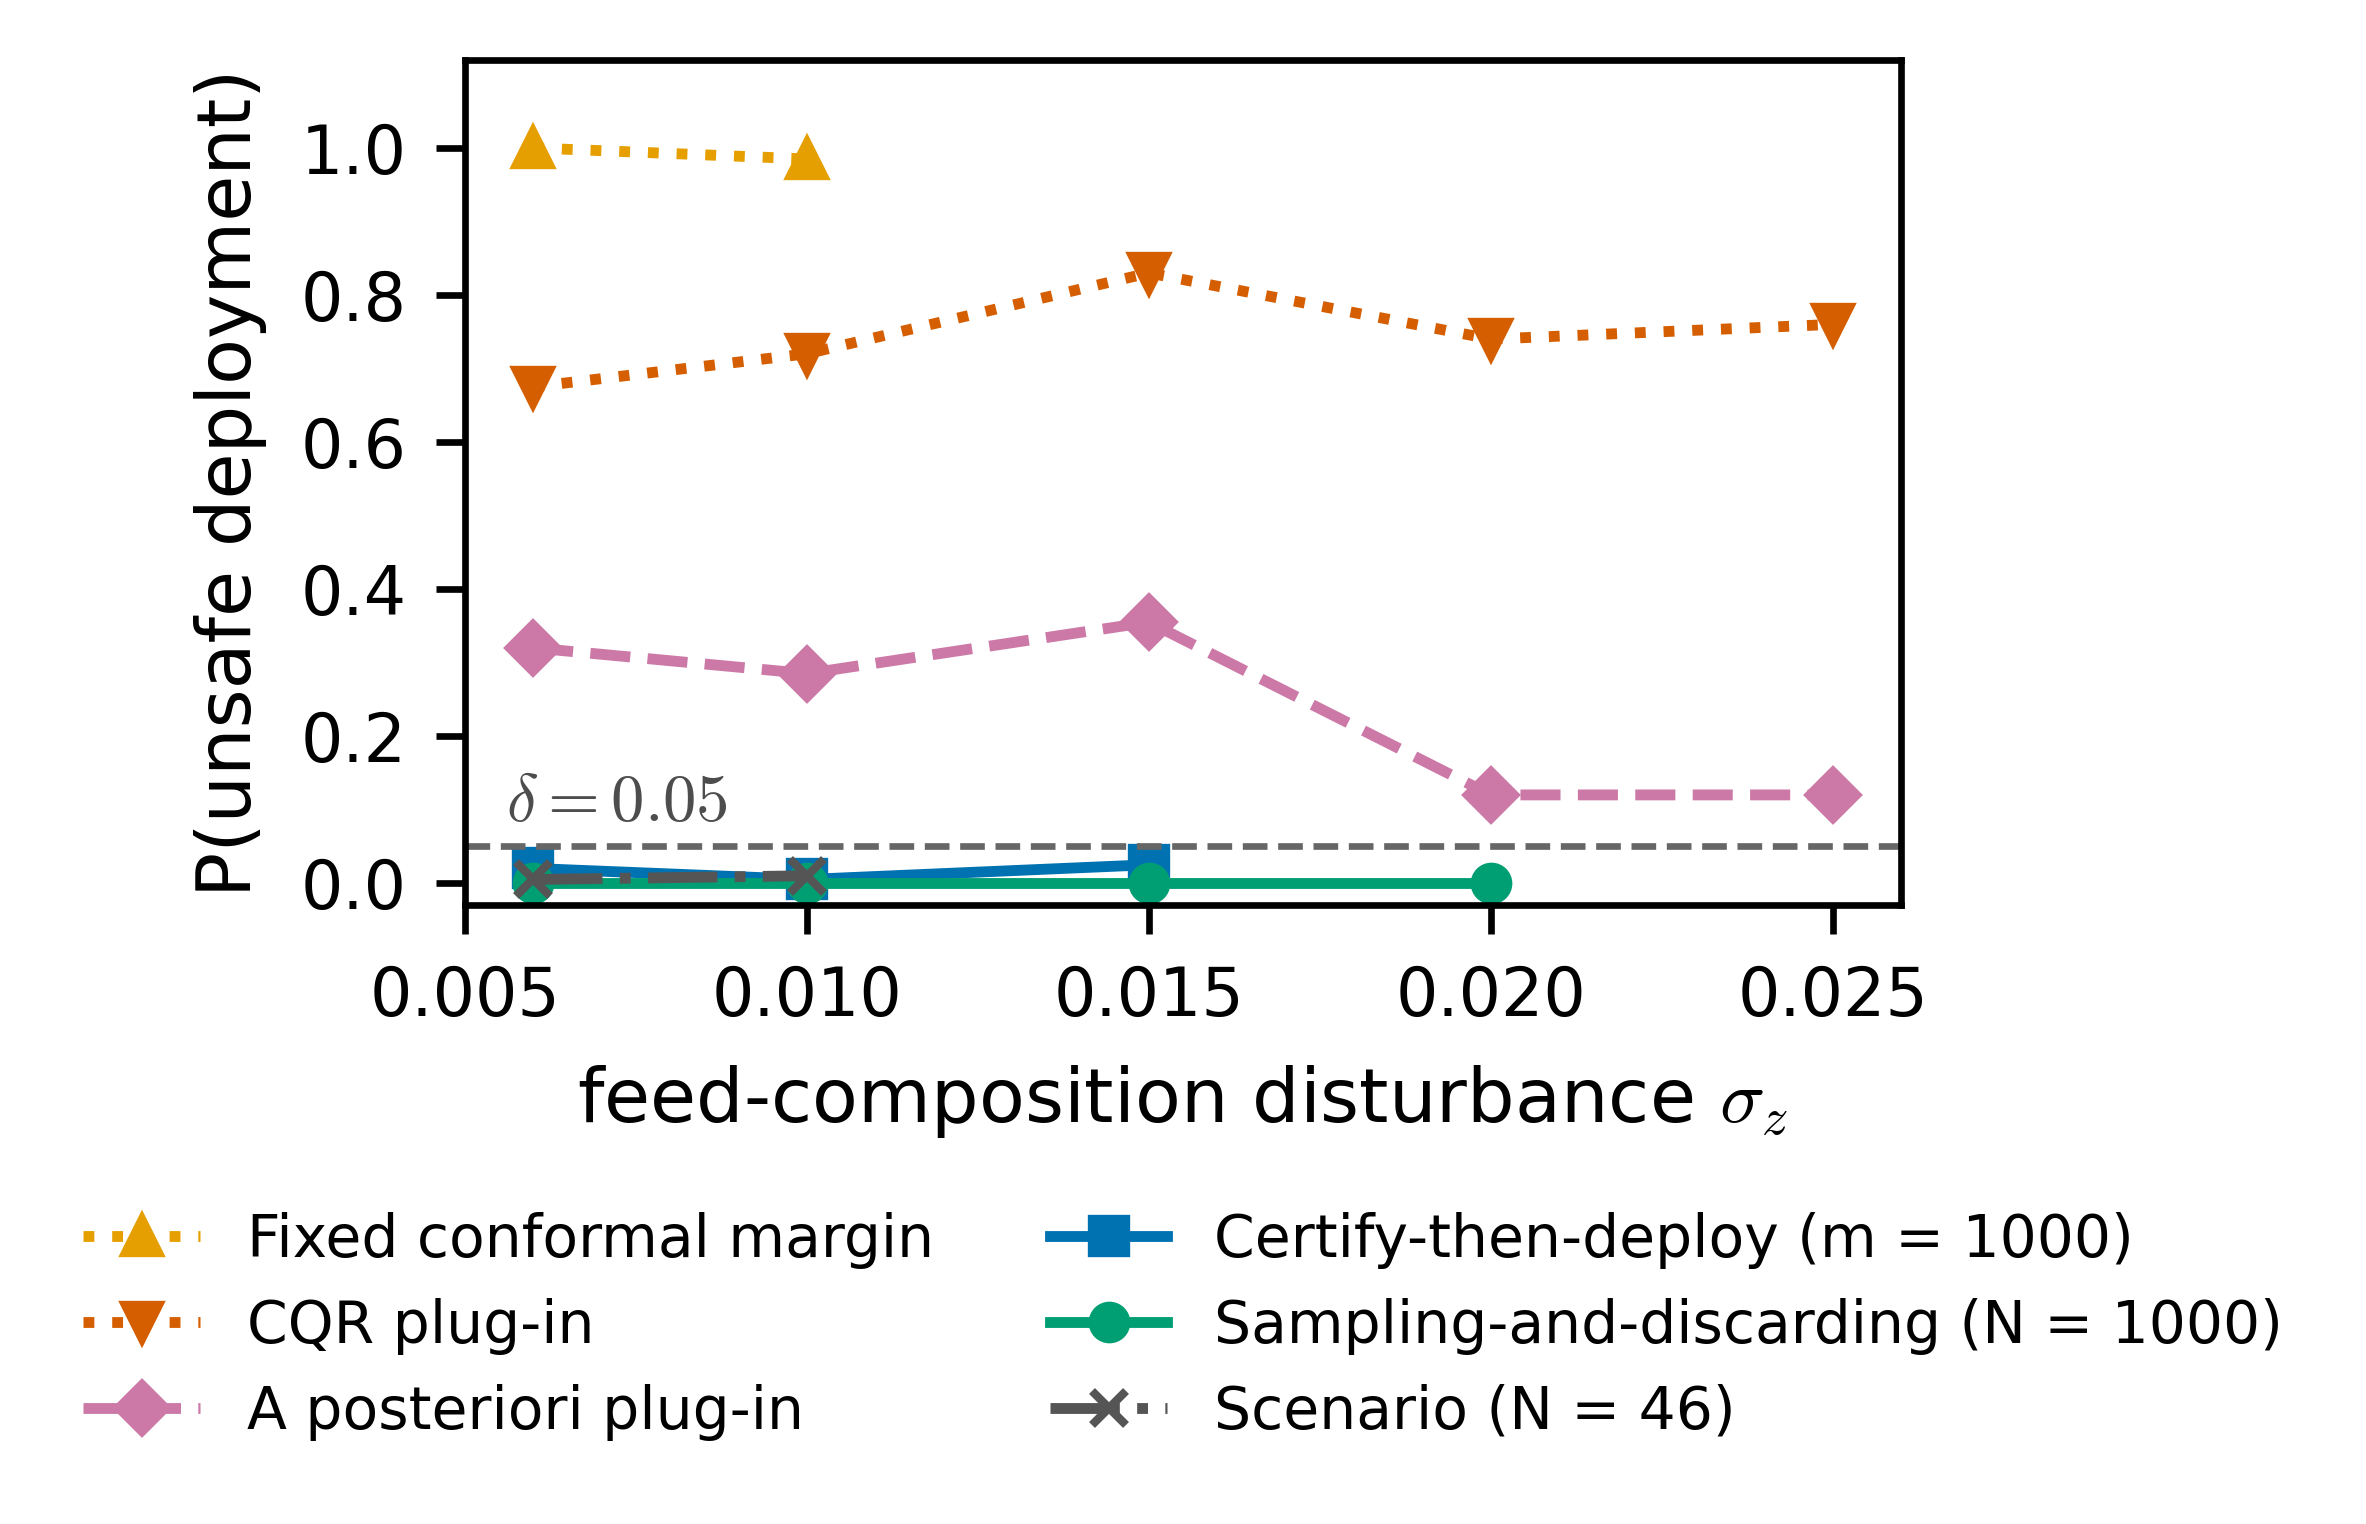
\includegraphics[width=0.62\textwidth]{fig_unsafe_vs_sigma.png}
\caption{Fraction of trials in which the deployed setpoint violates the specification with
probability above $\alpha = 0.10$, against the disturbance magnitude (200 trials per point; points
shown where the method deploys in at least half of the trials). The dashed line marks
$\delta = 0.05$.}
\label{fig:unsafe}
\end{figure}

\begin{table}[t]
\centering
\caption{Twin results at the realistic disturbance ($\sigma_z = 0.006$, 200 trials).}
\label{tab:main}
\small
\resizebox{\textwidth}{!}{\begin{tabular}{@{}lccccc@{}}
\toprule
\textbf{Method} & \textbf{Unsafe deployments (\%)} & \textbf{95\% CI (\%)} & \textbf{Deploys (\%)} & \textbf{$\Delta$profit (USD/h)} & \textbf{Mean $V$} \\
\midrule
Fixed conformal margin & 100.0 & 98.2 to 100 & 100 & $+7.5$ & 0.157 \\
CQR plug-in & 67.5 & 60.5 to 73.9 & 100 & $+4.5$ & 0.147 \\
A posteriori plug-in & 32.0 & 25.6 to 38.9 & 93 & $-4.1$ & 0.073 \\
Certify-then-deploy, $m=1000$ & 2.0 & 0.5 to 5.0 & 88 & $-11.5$ & 0.051 \\
Sampling-and-discarding, $N=1000$ & 0.0 & 0 to 1.8 & 100 & $-3.2$ & 0.064 \\
Scenario, $N=46$ & 0.5 & 0 to 2.8 & 100 & $-27.3$ & 0.020 \\
\bottomrule
\end{tabular}}

\vspace{2pt}
\parbox{\textwidth}{\footnotesize Note: $\Delta$profit is the expected profit minus the oracle profit
(5373.9 USD/h, $V = 0.083$, below 0.10 because of the finite grid); expected values include the
fallback setpoint for abstaining trials; CI, confidence interval; CQR, conformalized quantile regression.}
\end{table}

When the plant model fits inside the optimizer, sampling-and-discarding is the stronger method on
this problem: it is at least as safe as certify-then-deploy, it earns more (3.2 against 11.5 USD/h
below the oracle), and it never abstains for $\sigma_z \le 0.015$, whereas certify-then-deploy
abstains in 12\% of trials at the realistic level. With a single disturbance and a monotone response
only one sampled disturbance limits the solution, so discarding extracts almost all the information
in the samples. The basic scenario program with $N=46$ is safe but gives up 27.3 USD/h. All the
methods that meet Equation~\eqref{eq:pac} stay within 0.06\% to 0.21\% of the oracle profit; the differences
that matter are in safety, not in profit. Although conformal prediction and scenario optimization
are linked at the level of their guarantees,\citep{osullivan2025} the constructions compared here
certify different quantities: the marginal back-offs certify an average over calibration setpoints,
whereas certify-then-deploy and the scenario methods certify the setpoint that is deployed.

\subsection{Risk-adjusted economics}
The unguaranteed back-offs appear more profitable than the oracle because they operate beyond the
safe region. Equation \eqref{eq:J} puts a price on that. Figure~\ref{fig:econ} plots the
risk-adjusted profit relative to the oracle against the cost of off-spec bottoms. The fixed and CQR
back-offs lose their advantage over certify-then-deploy once off-spec bottoms cost more than 0.032
and 0.030 USD/kg, and over sampling-and-discarding above 0.021 and 0.017 USD/kg. These thresholds are
2\% to 4\% of the 0.836 USD/kg value of the product, so any disposition of off-spec gasoline that costs
more than a few percent of its value makes the guaranteed methods the better investment in
expectation. The a posteriori plug-in loses to certify-then-deploy above 0.060 USD/kg, and
sampling-and-discarding remains ahead of certify-then-deploy below 0.110 USD/kg.

\begin{figure}[t]
\centering
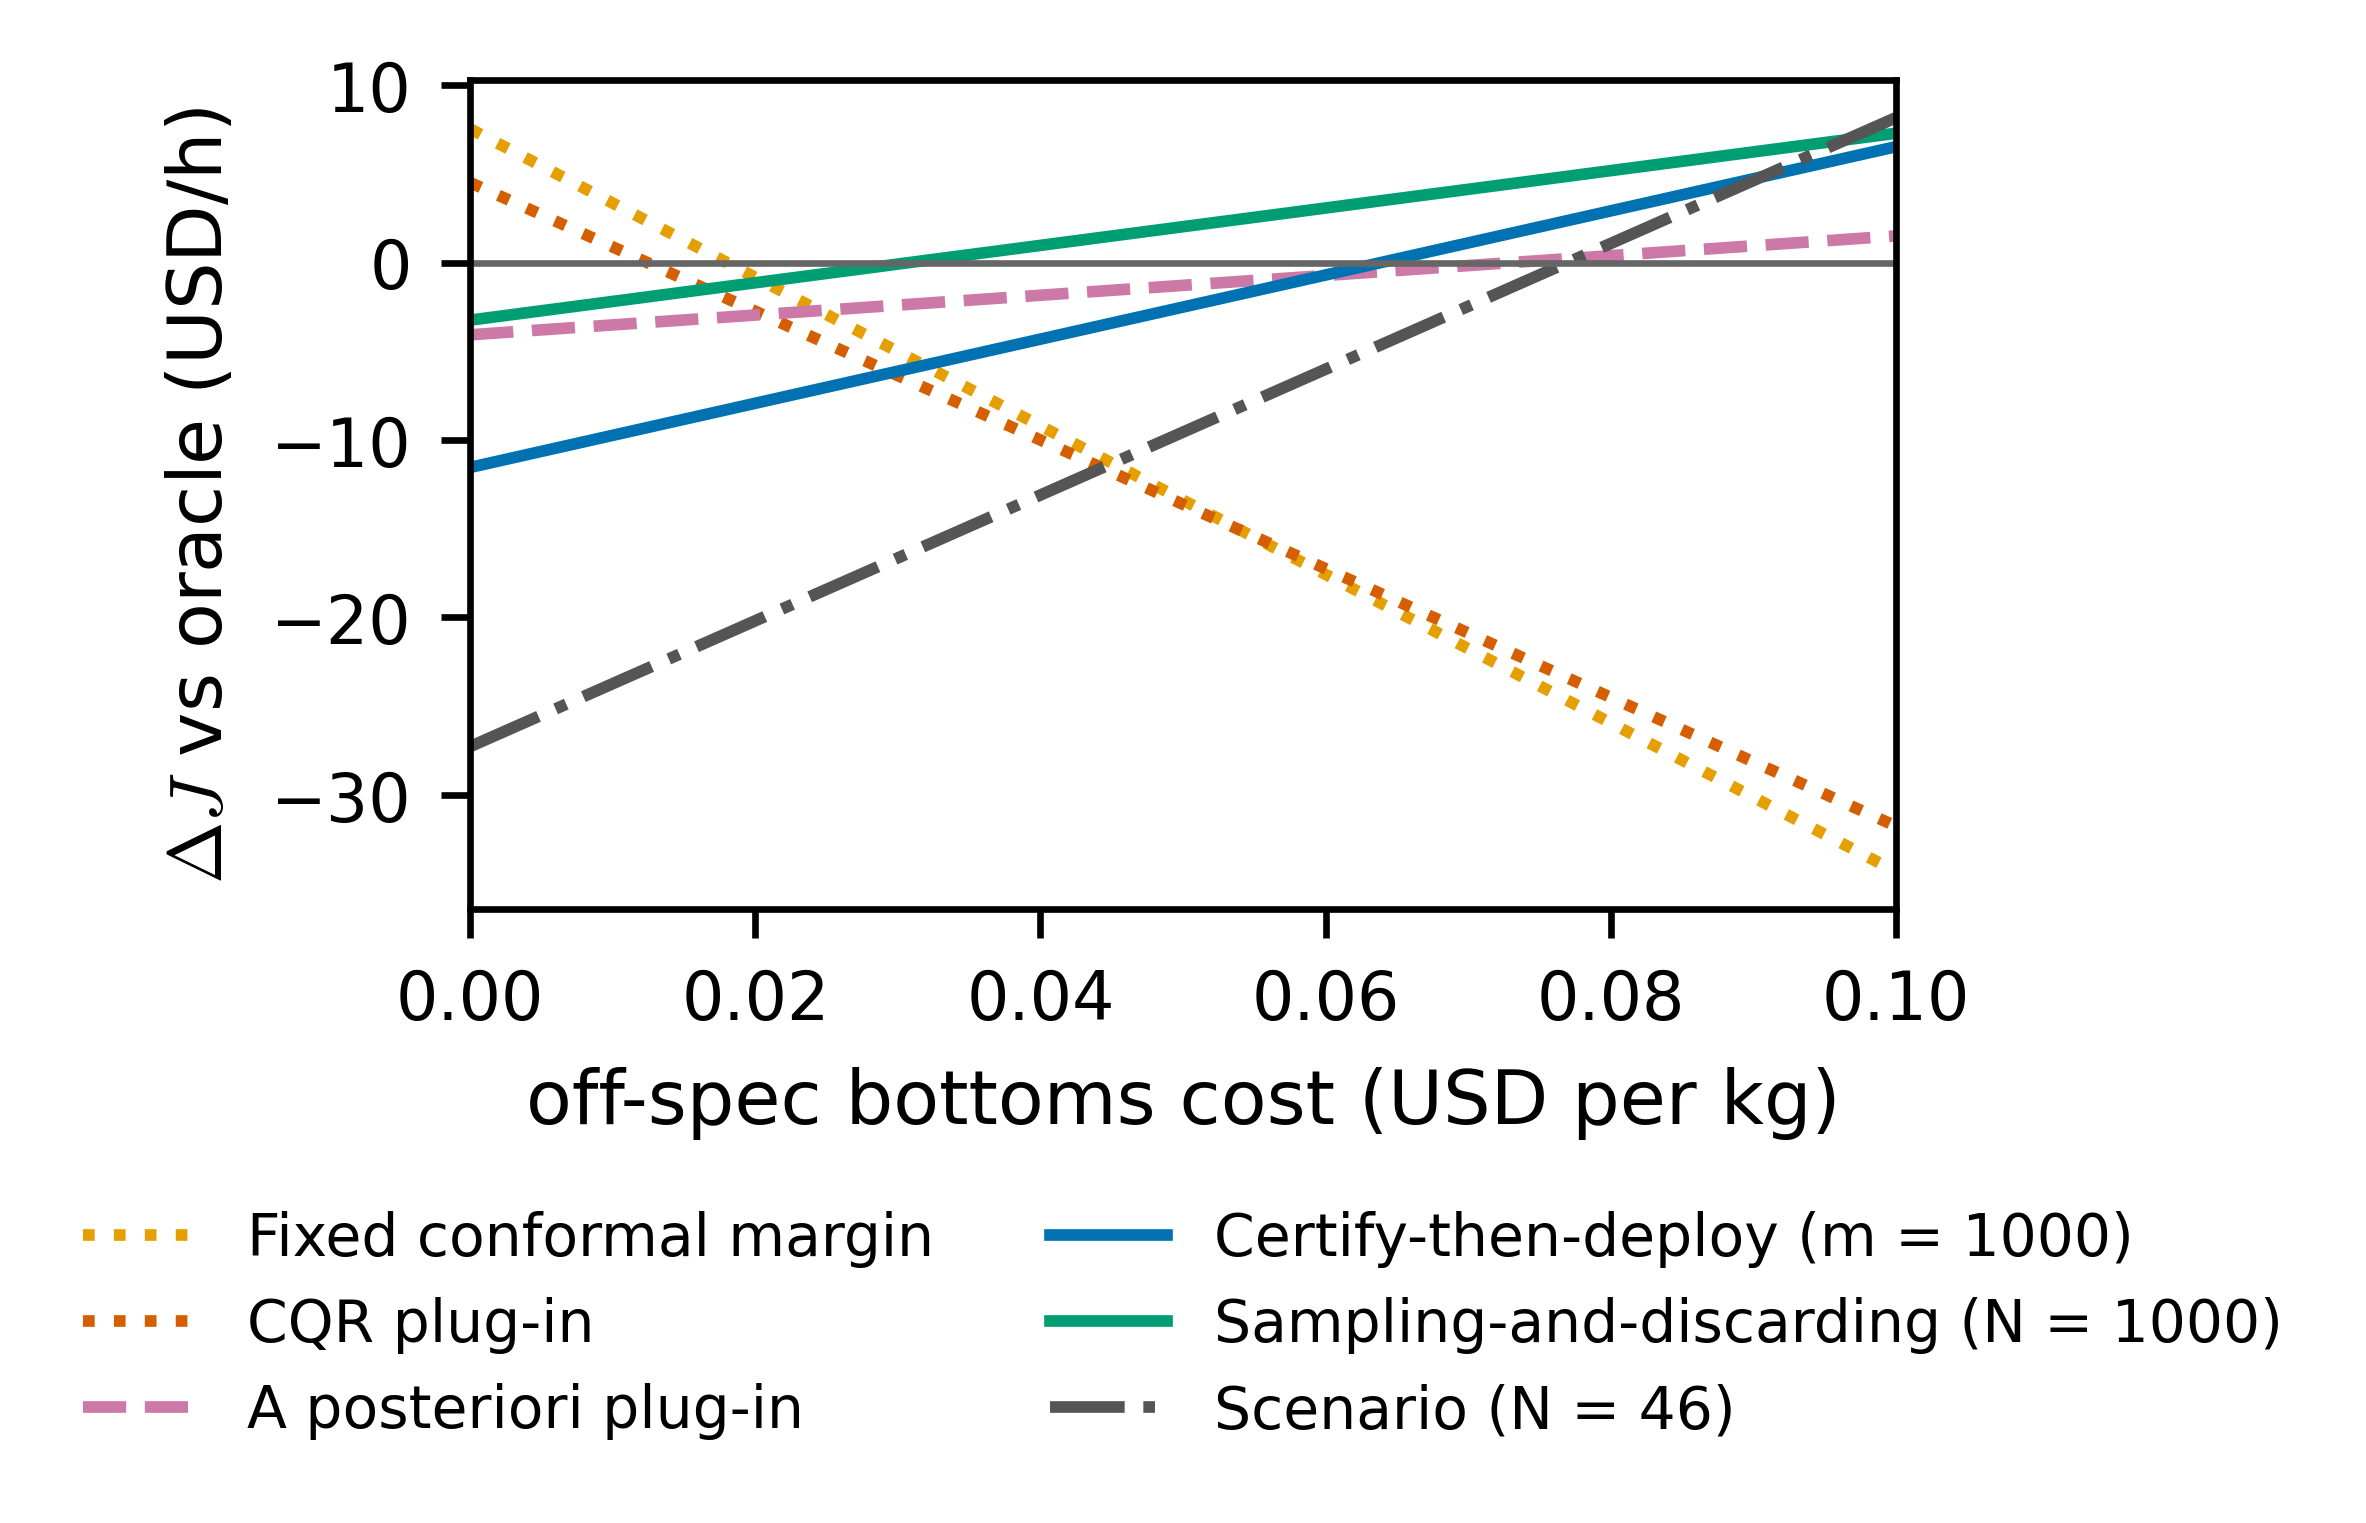
\includegraphics[width=0.62\textwidth]{fig_risk_adjusted_profit.png}
\caption{Expected risk-adjusted profit relative to the oracle, $\Delta J$, against the cost of
off-spec bottoms at $\sigma_z = 0.006$. Crossings mark the breakeven costs quoted in the text.}
\label{fig:econ}
\end{figure}

The same figure carries a second lesson. At off-spec costs above about 0.064 USD/kg even the
certified setpoint, which accepts $E(V) = 0.051$, earns more than the oracle designed for
$V = 0.10$, and above about 0.077 USD/kg so does the conservative scenario design. The chance level
$\alpha$ is therefore an economic decision rather than a convention: it should be set where the
marginal profit of relaxing the constraint equals the expected cost of the extra off-spec
production, and the procedures compared here can then enforce whatever level is chosen.

\subsection{Certification budget and abstention}
Certify-then-deploy needs enough samples to show that a candidate is safe. Figure~\ref{fig:budget}
gives the number of evaluations that certifies a candidate with 80\% probability as a function of its
true violation probability. A candidate that never violates needs 29 evaluations; one at 0.02 needs
61, at 0.04 needs 116, at 0.06 needs 286, and at 0.08 needs 1290. The budget grows steeply as the
candidate approaches $\alpha$, so a finite budget always deploys a setpoint strictly inside the safe
region. This is the price of the guarantee, and it is predictable before commissioning: an engineer
can choose $m$ from the figure and the profit gradient of the unit. When no candidate can be
certified the method abstains, which on the twin happens increasingly for $\sigma_z \ge 0.020$,
where the calibration data can no longer support a certified setpoint near the constraint. Abstaining
is the correct outcome in that regime: it signals that the disturbance has outgrown the data.

\begin{figure}[t]
\centering
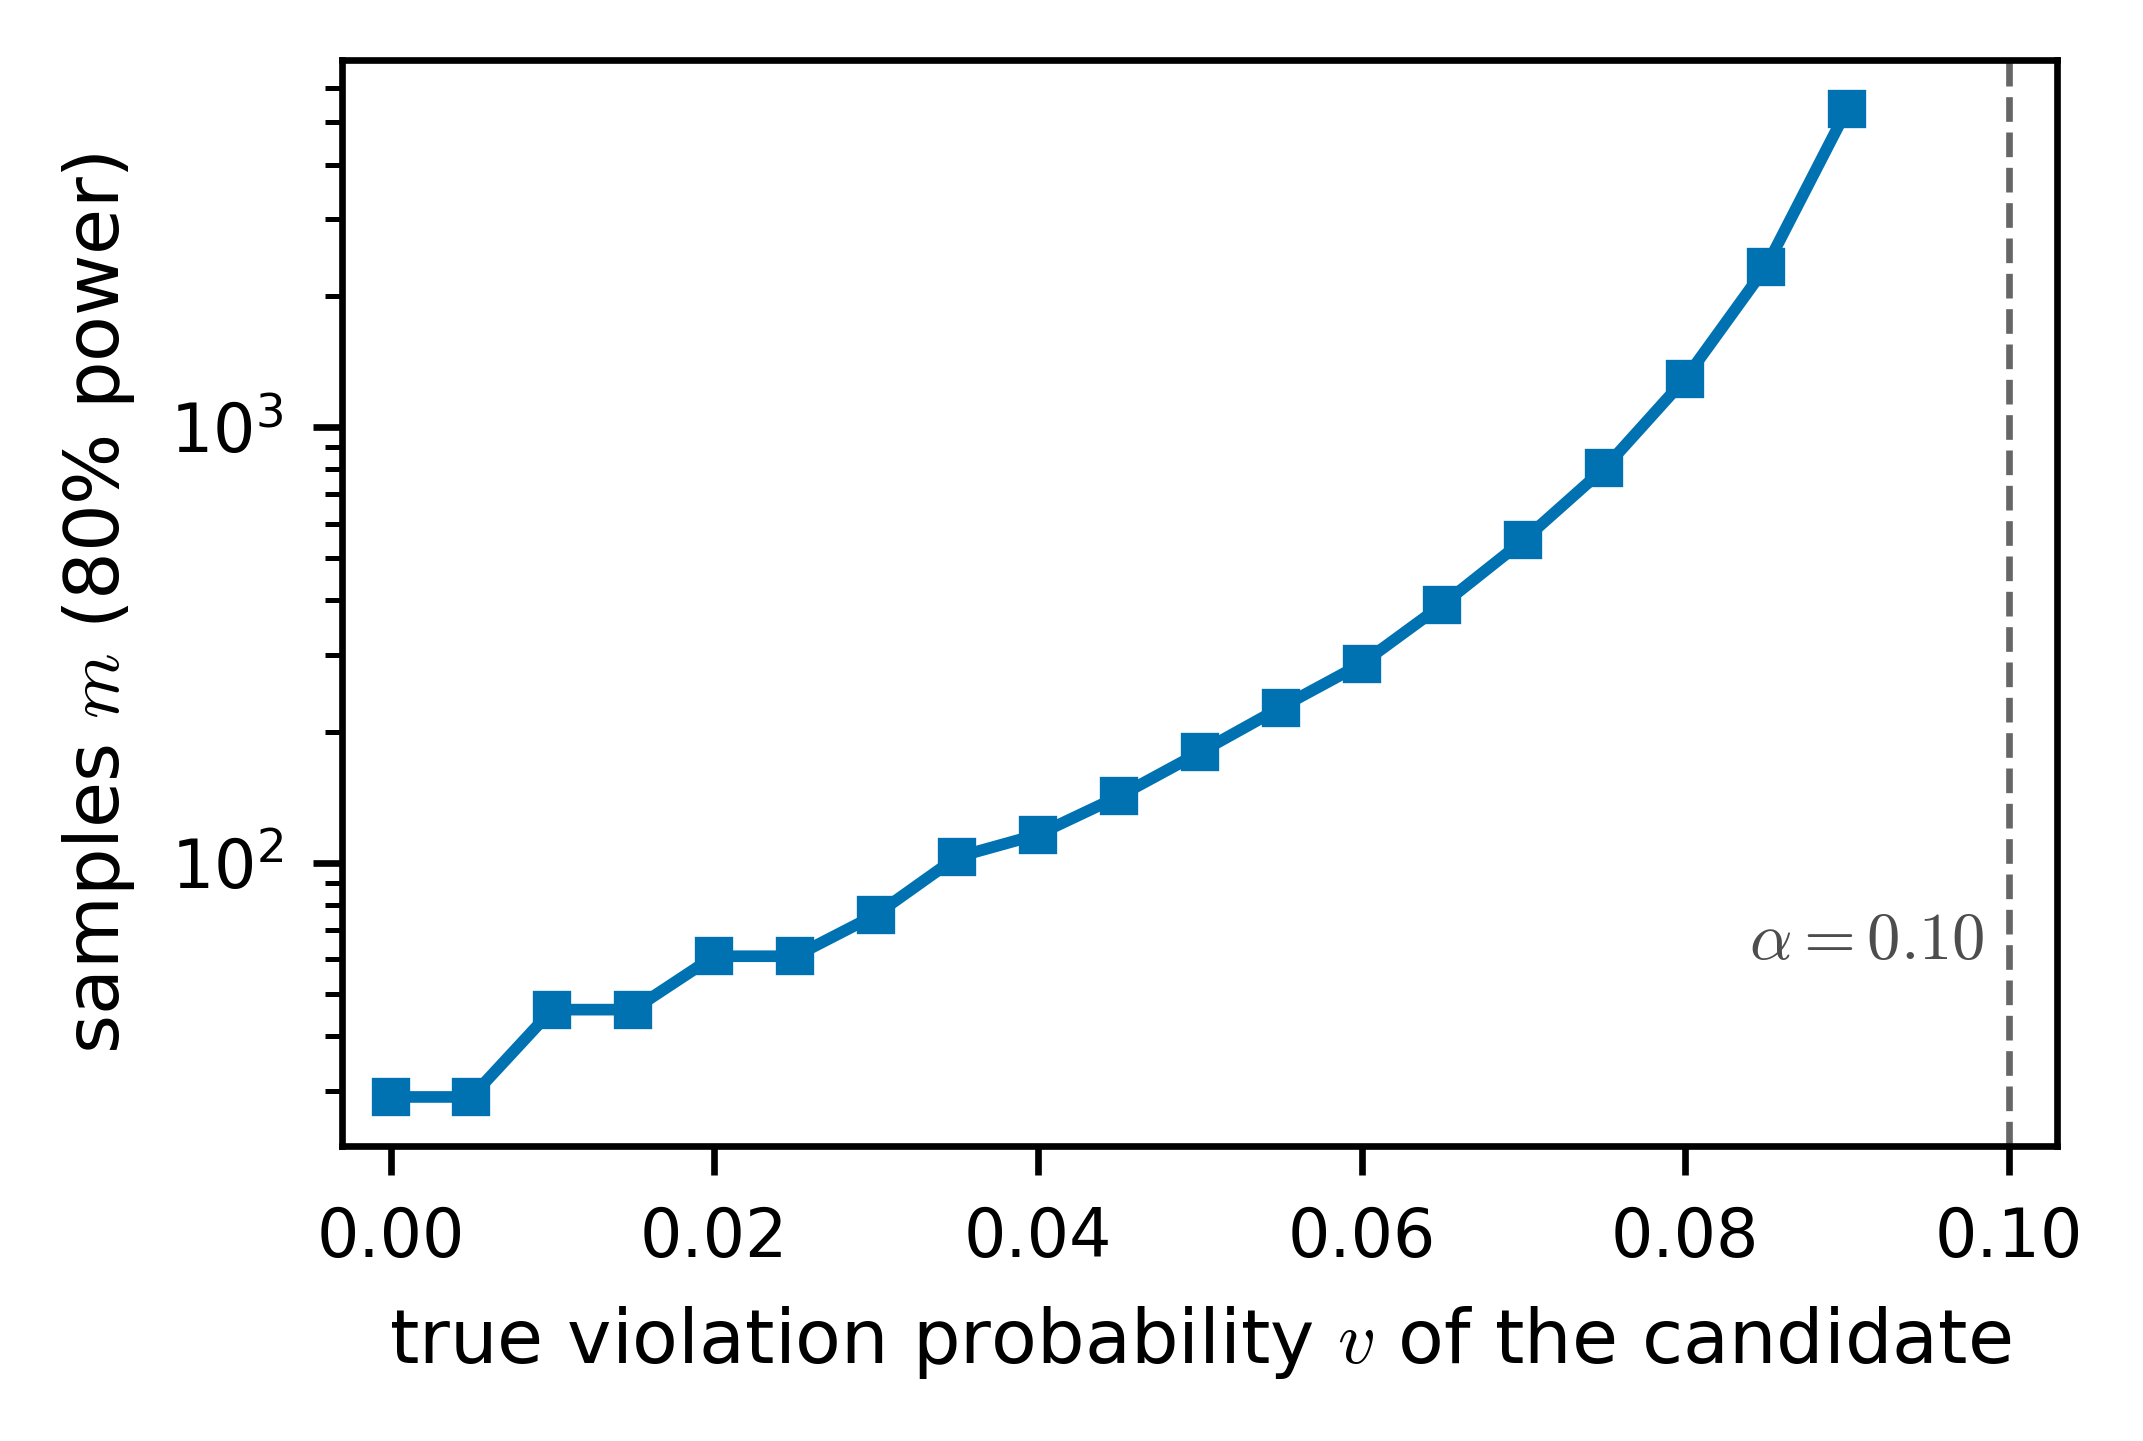
\includegraphics[width=0.62\textwidth]{fig_certification_budget.png}
\caption{Evaluations needed to certify a candidate setpoint with 80\% probability at
$\alpha = 0.10$ and $\delta = 0.05$, against its true violation probability.}
\label{fig:budget}
\end{figure}

\section{SELECTION GUIDE AND LIMITATIONS}

Table~\ref{tab:guide} condenses the evidence into a rule for choosing the back-off of a
chance-constrained RTO.

\begin{table}[t]
\centering
\caption{Choosing the back-off of a chance-constrained RTO.}
\label{tab:guide}
\small
\begin{tabular}{@{}>{\raggedright}p{0.36\textwidth}>{\raggedright}p{0.2\textwidth}>{\raggedright\arraybackslash}p{0.36\textwidth}@{}}
\toprule
\textbf{Situation} & \textbf{Use} & \textbf{Evidence} \\
\midrule
A validated plant model can be evaluated inside the optimizer & Sampling-and-discarding &
0.0\% unsafe deployments, 3.2 USD/h below the oracle, no abstention for $\sigma_z \le 0.015$ \\
The optimizer uses a nominal or surrogate model; the plant model or pilot runs can be evaluated at a
few candidate setpoints & Certify-then-deploy & At most 2.5\% unsafe deployments at every
disturbance level; budget from Figure~\ref{fig:budget}; valid for any optimizer \\
Only a marginally valid conformal back-off or a plug-in correction is available & Do not deploy
without certification & 12.0\% to 100\% unsafe deployments across disturbance levels \\
The chance level has not been fixed & Set $\alpha$ from the off-spec cost & Guaranteed methods
overtake the $\alpha=0.10$ oracle above 0.064 to 0.077 USD/kg \\
\bottomrule
\end{tabular}
\end{table}

The study has limits that bound these conclusions. The plant is a simulation twin, rigorous but not
an operating column, so the violation probabilities are relative to the twin, and the guarantees
of certify-then-deploy and the scenario methods hold with respect to the model used to evaluate
the candidates. The disturbance is a single scalar whose successive values are treated as
independent; real feed compositions drift and are autocorrelated, which breaks the independence
behind every guarantee compared here, and blocked or weighted certification is the natural next
step. With several disturbances or a non-monotone response more scenarios would limit the solution,
and the balance between sampling-and-discarding and certify-then-deploy may shift toward the latter,
whose sample size does not grow with the number of decision variables. Finally, the economic
thresholds depend on the price assumptions stated in Section 4 and scale with them.

\section{CONCLUSIONS}

Data-driven back-offs are a sound idea for RTO under unmeasured disturbances, but a back-off that
is valid on average is not safe at the setpoint an optimizer chooses. On a rigorous debutanizer twin,
conformal back-offs of this kind deployed a setpoint that exceeded the 10\% violation target in 67.5\%
to 100\% of trials, and a plug-in correction that is right on average still did so in 32.0\%.
Methods that check the deployed setpoint itself, certify-then-deploy and sampling-and-discarding,
kept this rate at or below 2.5\% for a profit cost of 0.06\% to 0.21\%, and they are the more profitable
choice in expectation whenever off-spec bottoms cost more than 2\% to 4\% of their value. The practical
rule is short: when the plant model can be evaluated inside the optimizer, use
sampling-and-discarding; when only a nominal model can, certify the candidate setpoints before
deploying them; and choose the chance level from the cost of off-spec product.

\section*{NOMENCLATURE}
\begingroup\small
\begin{tabular}{@{}p{0.13\textwidth}p{0.8\textwidth}@{}}
$C$ & back-off added to the nominal model ($-$) \\
$D$ & distillate molar flow rate (mol/s) \\
$g$ & bottoms \textit{n}-butane mole fraction, $x_B$ ($-$) \\
$\hat g$ & nominal model of $g$ at $z_0$ ($-$) \\
$\bar g$ & bottoms specification limit ($-$) \\
$J$ & risk-adjusted profit rate (USD/s) \\
$k$ & number of discarded scenarios ($-$) \\
$m$ & certification sample size ($-$) \\
$\dot m_B$ & bottoms mass flow rate (kg/s) \\
$n$ & calibration sample size ($-$) \\
$N$ & number of sampled scenarios ($-$) \\
$N_j$ & violation count of candidate $j$ ($-$) \\
$R$ & reflux ratio ($-$) \\
$U_j$ & Clopper-Pearson upper bound for candidate $j$ ($-$) \\
$u$ & decision vector, $(R, D)$ \\
$V$ & violation probability of a setpoint ($-$) \\
$x_B$ & bottoms \textit{n}-butane mole fraction ($-$) \\
$z$, $z_0$ & feed \textit{n}-butane mole fraction and its nominal value ($-$) \\
\end{tabular}

\medskip\noindent\textit{Greek Letters}\\[2pt]
\begin{tabular}{@{}p{0.13\textwidth}p{0.8\textwidth}@{}}
$\alpha$ & chance-constraint level ($-$) \\
$\delta$ & allowed probability of deploying an unsafe setpoint ($-$) \\
$\Delta$ & cost of off-spec bottoms per unit mass (USD/kg) \\
$\kappa$ & back-off inflation factor ($-$) \\
$\pi$ & operating profit rate (USD/s) \\
$\sigma_z$ & standard deviation of the feed composition ($-$) \\
\end{tabular}
\endgroup

\section*{AUTHOR CONTRIBUTIONS}
\textbf{Bien Don Busico:} Conceptualization; data curation; formal analysis; investigation;
methodology; project administration; resources; software; validation; visualization; writing,
original draft; writing, review and editing.

\section*{FUNDING INFORMATION}
This research received no specific grant from any funding agency in the public, commercial, or
not-for-profit sectors.

\section*{CONFLICT OF INTEREST STATEMENT}
The author declares no conflict of interest.

\section*{DATA AVAILABILITY STATEMENT}
The data that support the findings of this study are openly available in GitHub at
\url{https://github.com/beebzy-droid/IPIS}, including the DWSIM campaign data
(\url{docs/module3/cjce/data}), the scripts that regenerate every figure and table from fixed random
seeds, and the evidence files.

\bibliographystyle{angew}
\bibliography{references}

\end{document}
